\documentclass[tikz,border=8pt]{standalone}

\usepackage[T1]{fontenc}
\usepackage{lmodern}
\usetikzlibrary{arrows.meta,backgrounds,calc,positioning,fit,shapes.geometric}

\definecolor{flowblue}{HTML}{0072B2}
\definecolor{flowgreen}{HTML}{009E73}
\definecolor{flowbrown}{HTML}{8C564B}
\definecolor{flowpurple}{HTML}{6F4EA1}
\definecolor{floworange}{HTML}{D55E00}
\definecolor{ink}{HTML}{243447}
\definecolor{mutedink}{HTML}{52606D}
\definecolor{linegray}{HTML}{9AA5B1}
\definecolor{panel}{HTML}{F5F7FA}
\definecolor{ownedfill}{HTML}{E8F1F8}
\definecolor{storefill}{HTML}{FFF1CC}
\definecolor{externalfill}{HTML}{F3ECF8}

\tikzset{
  box/.style={
    draw=linegray,
    fill=white,
    rounded corners=2pt,
    line width=0.6pt,
    minimum height=10mm,
    text width=30mm,
    align=center,
    font=\sffamily\small,
    text=ink,
    inner sep=4pt
  },
  actor/.style={box,text width=24mm},
  component/.style={box,fill=ownedfill},
  store/.style={box,fill=storefill,text width=24mm},
  external/.style={box,fill=externalfill,text width=34mm},
  network/.style={box,text width=26mm},
  boundary title/.style={font=\sffamily\bfseries\large,text=ink,anchor=west},
  flow/.style={-{Latex[length=3mm,width=2.2mm]},line width=1.6pt},
  story one/.style={flow,draw=flowblue},
  story two/.style={flow,draw=flowgreen},
  story three/.style={flow,draw=flowbrown},
  story four/.style={flow,draw=flowpurple},
  story five/.style={flow,draw=floworange},
  relation/.style={draw=linegray,line width=1.1pt},
  edge label/.style={
    fill=none,
    inner xsep=1.5pt,
    inner ysep=3pt,
    font=\sffamily\scriptsize,
    text=mutedink,
    align=center
  },
  every node/.append style={font=\sffamily}
}

\newcommand{\storyStep}[2]{%
  \tikz[baseline=(step.base)]
    \node[circle,fill=#1,text=white,inner sep=1.1pt,
      font=\sffamily\bfseries\tiny] (step) {#2};%
}


\tikzset{
  dependency/.style={relation,-{Latex[length=2.3mm,width=1.6mm]}},
  planned/.style={component,dashed,fill=white},
  smallbox/.style={component,text width=27mm,minimum height=10mm},
  table/.style={box,align=left,text width=50mm,inner sep=7pt,font=\sffamily\small},
  fk/.style={relation,-{Latex[length=2.6mm]},draw=ink,line width=1.2pt},
  logical/.style={relation,-{Latex[length=2.6mm]},draw=flowblue,dashed,line width=1.2pt},
  note/.style={font=\sffamily\small,text=mutedink,align=left},
  title/.style={font=\sffamily\bfseries\Large,text=ink,anchor=west}
}

\begin{document}
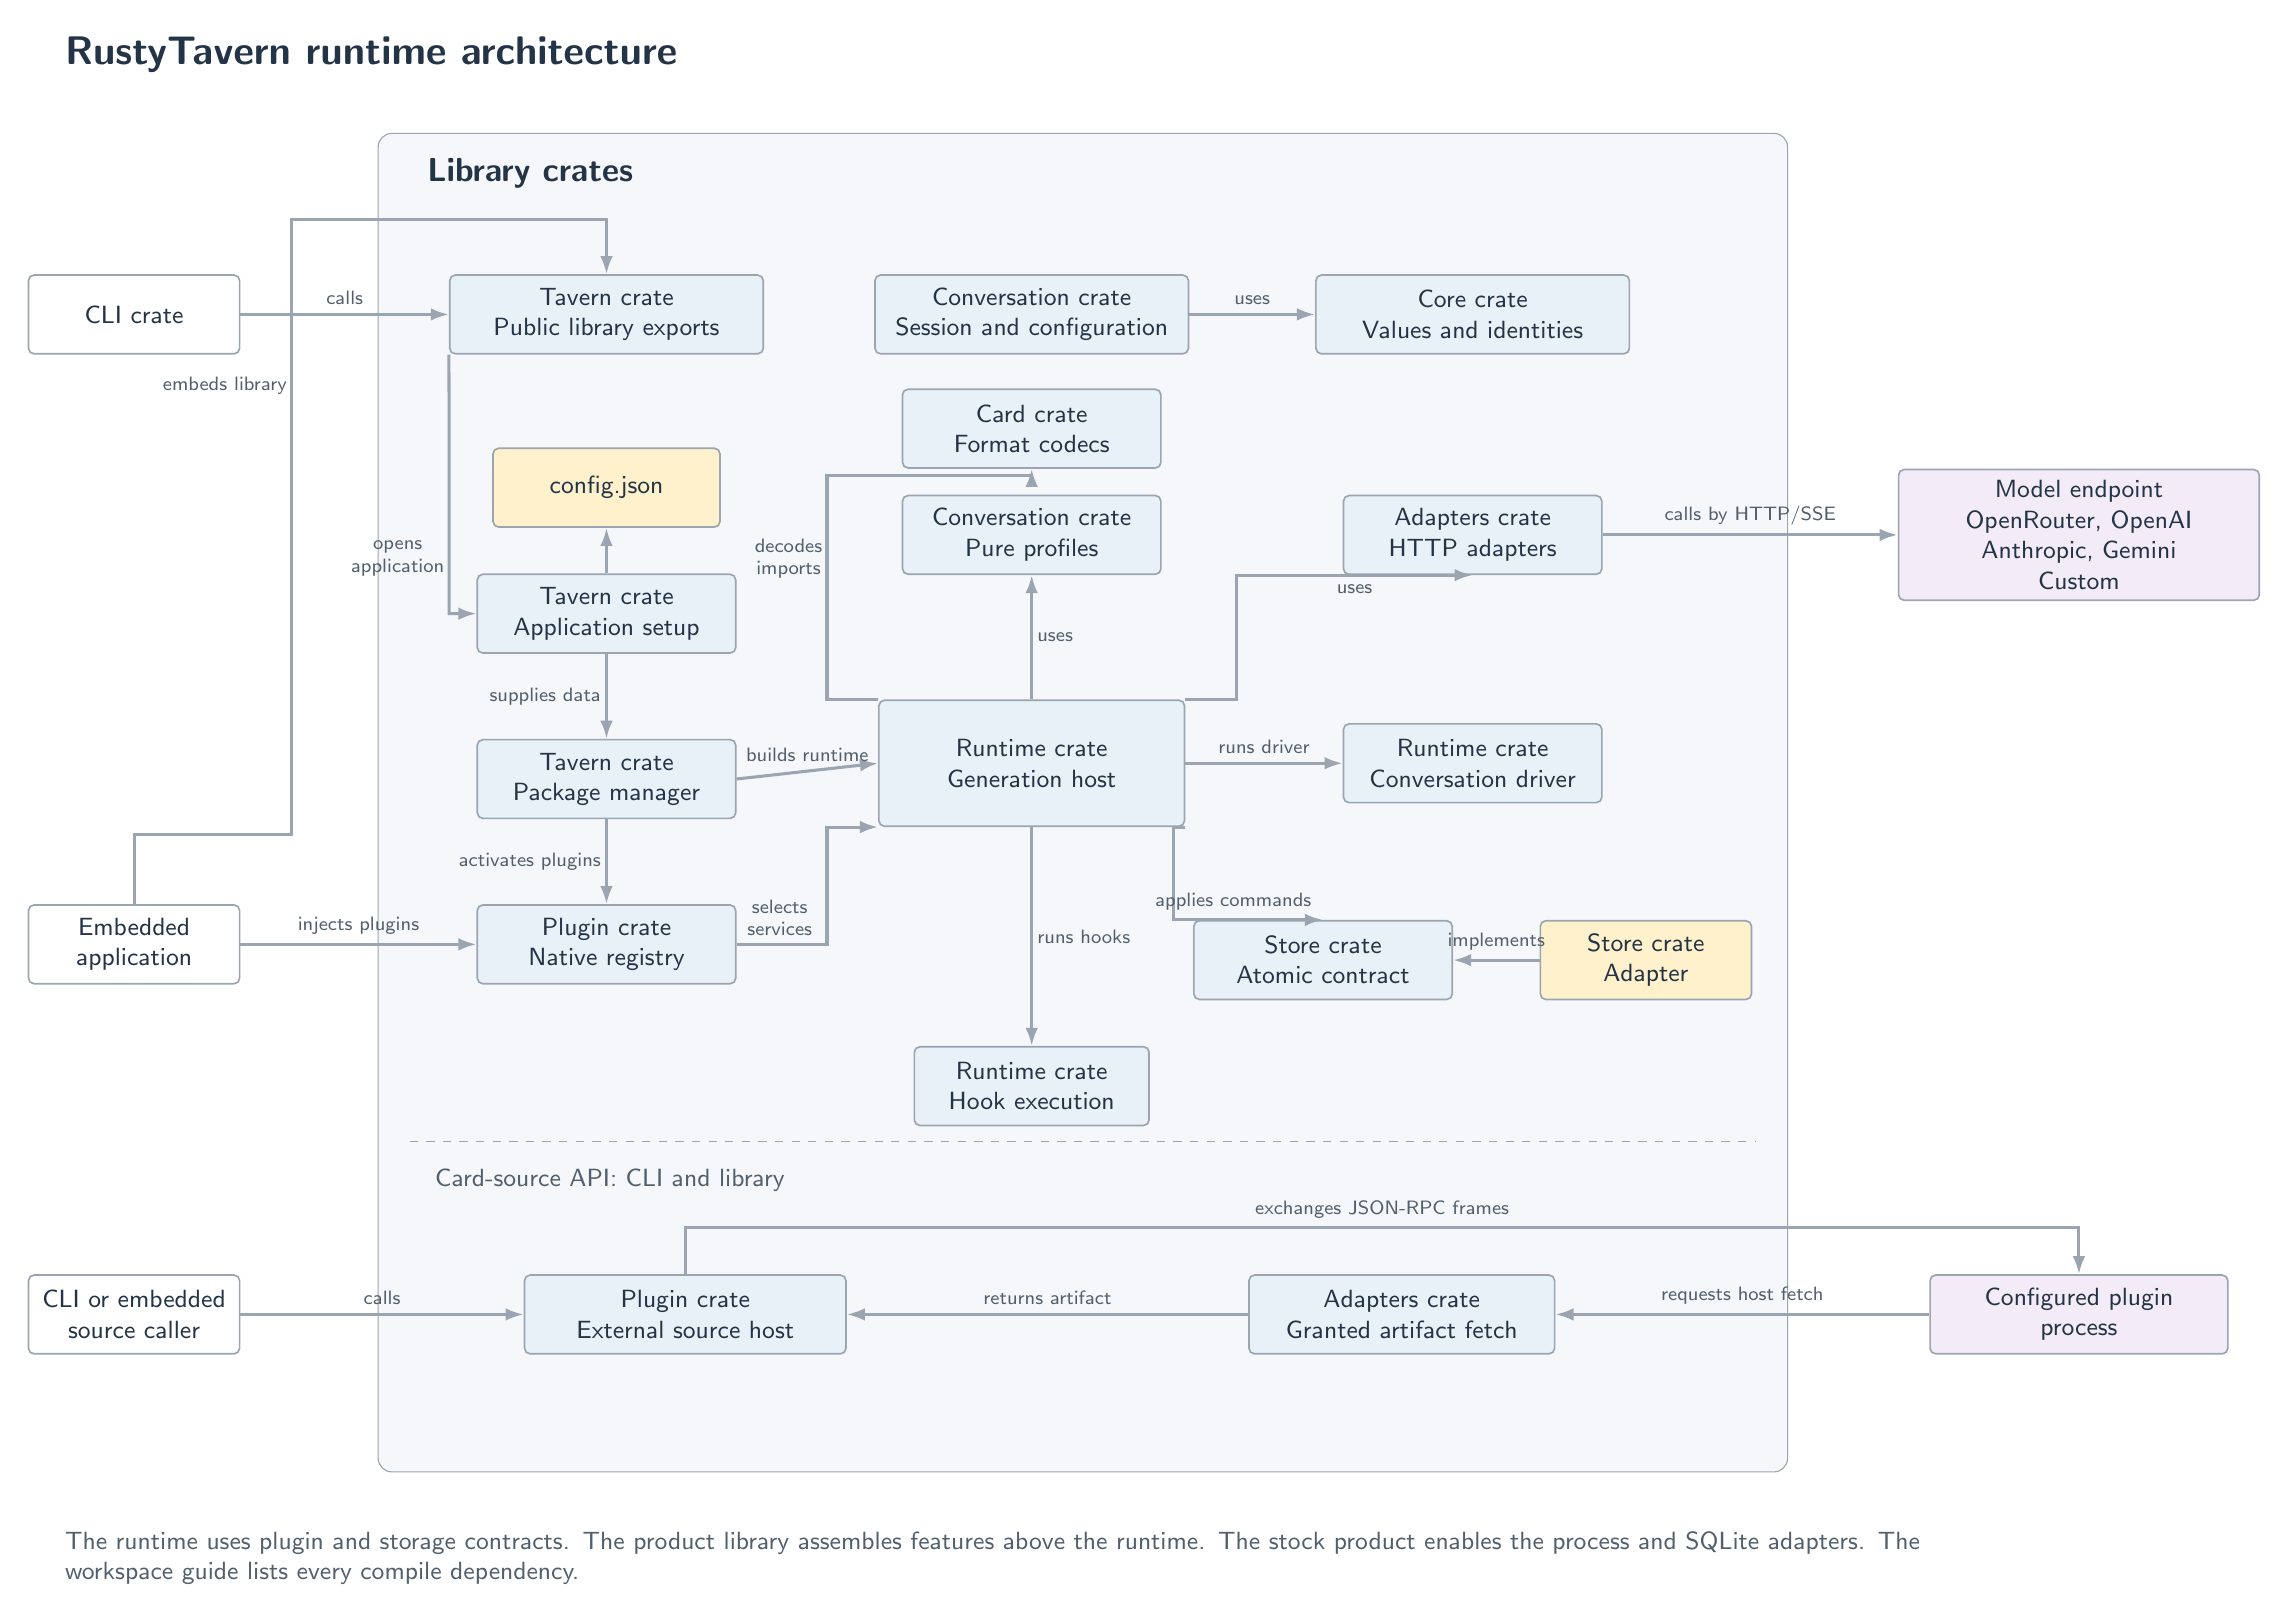
\begin{tikzpicture}[x=1cm,y=1cm]

\node[title] at (-1,18) {RustyTavern runtime architecture};
\begin{scope}[on background layer]
  \filldraw[fill=panel,draw=linegray,rounded corners=5pt] (3.1,0) rectangle (21,17);
  \draw[linegray,dashed] (3.5,4.2) -- (20.6,4.2);
\end{scope}
\node[boundary title] at (3.6,16.5) {Library crates};
\node[actor] (cli) at (0,14.7) {CLI crate};
\node[actor] (embed) at (0,6.7) {Embedded\\application};
\node[component] (config) at (6,10.9) {Tavern crate\\Application setup};
\node[component] (manager) at (6,8.8) {Tavern crate\\Package manager};
\node[component,text width=36mm,minimum height=16mm] (host) at (11.4,9.0) {Runtime crate\\Generation host};
\node[component] (profile) at (11.4,11.9) {Conversation crate\\Pure profiles};
\node[component] (decoder) at (11.4,13.25) {Card crate\\Format codecs};
\node[component] (driver) at (17,9.0) {Runtime crate\\Conversation driver};
\node[component] (adapter) at (17,11.9) {Adapters crate\\HTTP adapters};
\node[external,text width=43mm] (models) at (24.7,11.9) {Model endpoint\\OpenRouter, OpenAI\\Anthropic, Gemini\\Custom};
\node[component] (registry) at (6,6.7) {Plugin crate\\Native registry};
\node[component,text width=27mm] (phases) at (11.4,4.9) {Runtime crate\\Hook execution};
\node[component] (backend) at (15.1,6.5) {Store crate\\Atomic contract};
\node[store] (db) at (19.2,6.5) {Store crate\\Adapter};
\node[store,text width=26mm] (cfg) at (6,12.5) {config.json};
\node[component,text width=37mm] (facade) at (6,14.7) {Tavern crate\\Public library exports};
\node[component,text width=37mm] (records) at (11.4,14.7) {Conversation crate\\Session and configuration};
\node[component,text width=37mm] (core) at (17,14.7) {Core crate\\Values and identities};
\draw[dependency] (cli.east) -- node[edge label,above] {calls} (facade.west);
\draw[dependency] (facade.south west) -- (4,13.7) |- (config.west);
\node[edge label,left] at (4,11.6) {opens\\application};
\draw[dependency] (embed.north) -- (0,8.1) -- (2,8.1) -- (2,15.9) -- (6,15.9) -- (facade.north);
\node[edge label,left] at (2,13.8) {embeds library};
\draw[dependency] (config.south) -- node[edge label,left] {supplies data} (manager.north);
\draw[dependency] (manager.south) -- node[edge label,left] {activates plugins} (registry.north);
\draw[dependency] (manager.east) -- node[edge label,above] {builds runtime} (host.west);
\draw[dependency] (config.north) -- (cfg.south);
\draw[dependency] (embed.east) -- node[edge label,above] {injects plugins} (registry.west);
\draw[dependency] (registry.east) -- (8.8,6.7) |- (host.south west);
\node[edge label,above] at (8.2,6.7) {selects\\services};
\draw[dependency] (host.south) -- node[edge label,right] {runs hooks} (phases.north);
\draw[dependency] (host.north west) -| (8.8,12.65) -| (decoder.south);
\node[edge label,left] at (8.8,11.6) {decodes\\imports};
\draw[dependency] (host.east) -- node[edge label,above] {runs driver} (driver.west);
\draw[dependency] (host.north) -- node[edge label,right] {uses} (profile.south);
\draw[dependency] (host.north east) -| (14,10.2) |- node[edge label,pos=.75,below] {uses} (adapter.south);
\draw[dependency] (adapter.east) -- node[edge label,above] {calls by HTTP/SSE} (models.west);
\draw[dependency] (host.south east) -| (13.2,7.8) |- node[edge label,pos=.7,above] {applies commands} (backend.north);
\draw[dependency] (db.west) -- node[edge label,above] {implements} (backend.east);
\node[note,anchor=west] at (3.7,3.7) {Card-source API: CLI and library};
\node[actor] (sourcecaller) at (0,2) {CLI or embedded\\source caller};
\node[component,text width=38mm] (rpc) at (7,2) {Plugin crate\\External source host};
\node[component,text width=36mm] (fetch) at (16.1,2) {Adapters crate\\Granted artifact fetch};
\node[external,text width=35mm] (process) at (24.7,2) {Configured plugin\\process};
\draw[dependency] (sourcecaller.east) -- node[edge label,above] {calls} (rpc.west);
\draw[dependency] (rpc.north) -- (7,3.1) -- node[edge label,above] {exchanges JSON-RPC frames} (24.7,3.1) -- (process.north);
\draw[dependency] (process.west) -- node[edge label,above] {requests host fetch} (fetch.east);
\draw[dependency] (fetch.west) -- node[edge label,above] {returns artifact} (rpc.east);
\draw[dependency] (records.east) -- node[edge label,above] {uses} (core.west);
\node[note,anchor=west,text width=245mm] at (-1,-1.1) {The runtime uses plugin and storage contracts. The product library assembles features above the runtime. The stock product enables the process and SQLite adapters. The workspace guide lists every compile dependency.};

\end{tikzpicture}
\end{document}
